\documentclass[11pt,letterpaper]{article}
\usepackage[utf8]{inputenc}
\usepackage{caption} % for table captions
\usepackage{amsmath} % for multi-line equations and piecewises
\DeclareMathOperator{\sign}{sign}
\usepackage{graphicx}
\usepackage{relsize}
%\usepackage{textcomp}
\usepackage{xspace}
\usepackage{verbatim} % for block comments
%\usepackage{subfig} % for subfigures
\usepackage{enumitem} % for a) b) c) lists
\newcommand{\Cyclus}{\textsc{Cyclus}\xspace}%
\newcommand{\Cycamore}{\textsc{Cycamore}\xspace}%
\usepackage{tabularx}
\usepackage{color}
\usepackage[acronym,toc]{glossaries}
%\newacronym{<++>}{<++>}{<++>}
%\newacronym{<++>}{<++>}{<++>}
\newacronym[longplural={metric tons of heavy metal}]{MTHM}{MTHM}{metric ton of heavy metal}
\newacronym{ABM}{ABM}{agent-based modeling}
\newacronym{AHTR}{AHTR}{Advanced High Temperature Reactor}
\newacronym{ANDRA}{ANDRA}{Agence Nationale pour la gestion des D\'echets RAdioactifs, the French National Agency for Radioactive Waste Management}
\newacronym{ANL}{ANL}{Argonne National Laboratory}
\newacronym{API}{API}{application programming interface}
\newacronym{ARCH}{ARCH}{autoregressive conditional heteroskedastic}
\newacronym{ARE}{ARE}{Aircraft Reactor Experiment}
\newacronym{ARFC}{ARFC}{Advanced Reactors and Fuel Cycles}
\newacronym{ARMA}{ARMA}{autoregressive moving average}
\newacronym{ASME}{ASME}{American Society of Mechanical Engineers}
\newacronym{ATWS}{ATWS}{Anticipated Transient Without Scram}
\newacronym{BDBE}{BDBE}{Beyond Design Basis Event}
\newacronym{BIDS}{BIDS}{Berkeley Institute for Data Science}
\newacronym{CAFCA}{CAFCA}{ Code for Advanced Fuel Cycles Assessment }
\newacronym{CEA}{CEA}{Commissariat \`a l'\'Energie Atomique et aux \'Energies Alternatives}
\newacronym{CI}{CI}{continuous integration}
\newacronym{CNERG}{CNERG}{Computational Nuclear Engineering Research Group}
\newacronym{COSI}{COSI}{Commelini-Sicard}
\newacronym{COTS}{COTS}{commercial, off-the-shelf}
\newacronym{CSNF}{CSNF}{commercial spent nuclear fuel}
\newacronym{CTAH}{CTAHs}{Coiled Tube Air Heaters}
\newacronym{CUBIT}{CUBIT}{CUBIT Geometry and Mesh Generation Toolkit}
\newacronym{DAG}{DAG}{directed acyclic graph}
\newacronym{DANESS}{DANESS}{Dynamic Analysis of Nuclear Energy System Strategies}
\newacronym{DBE}{DBE}{Design Basis Event}
\newacronym{DESAE}{DESAE}{Dynamic Analysis of Nuclear Energy Systems Strategies}
\newacronym{DHS}{DHS}{Department of Homeland Security}
\newacronym{DOE}{DOE}{Department of Energy}
\newacronym{DRACS}{DRACS}{Direct Reactor Auxiliary Cooling System}
\newacronym{DRE}{DRE}{dynamic resource exchange}
\newacronym{DSNF}{DSNF}{DOE spent nuclear fuel}
\newacronym{DYMOND}{DYMOND}{Dynamic Model of Nuclear Development }
\newacronym{EBS}{EBS}{Engineered Barrier System}
\newacronym{EDZ}{EDZ}{Excavation Disturbed Zone}
\newacronym{EPA}{EPA}{Environmental Protection Agency}
\newacronym{EP}{EP}{Engineering Physics}
\newacronym{FCO}{FCO}{Fuel Cycle Options}
\newacronym{FCT}{FCT}{Fuel Cycle Technology}
\newacronym{FEHM}{FEHM}{Finite Element Heat and Mass Transfer}
\newacronym{FEPs}{FEPs}{Features, Events, and Processes}
\newacronym{FHR}{FHR}{Fluoride-Salt-Cooled High-Temperature Reactor}
\newacronym{FLiBe}{FLiBe}{Fluoride-Lithium-Beryllium}
\newacronym{GCAM}{GCAM}{Global Change Assessment Model}
\newacronym{GDSE}{GDSE}{Generic Disposal System Environment}
\newacronym{GDSM}{GDSM}{Generic Disposal System Model}
\newacronym{GENIUSv1}{GENIUSv1}{Global Evaluation of Nuclear Infrastructure Utilization Scenarios, Version 1}
\newacronym{GENIUSv2}{GENIUSv2}{Global Evaluation of Nuclear Infrastructure Utilization Scenarios, Version 2}
\newacronym{GENIUS}{GENIUS}{Global Evaluation of Nuclear Infrastructure Utilization Scenarios}
\newacronym{GPAM}{GPAM}{Generic Performance Assessment Model}
\newacronym{GRSAC}{GRSAC}{Graphite Reactor Severe Accident Code}
\newacronym{GUI}{GUI}{graphical user interface}
\newacronym{HLW}{HLW}{high level waste}
\newacronym{HPC}{HPC}{high-performance computing}
\newacronym{HTC}{HTC}{high-throughput computing}
\newacronym{HTGR}{HTGR}{High Temperature Gas-Cooled Reactor}
\newacronym{IAEA}{IAEA}{International Atomic Energy Agency}
\newacronym{INL}{INL}{Idaho National Laboratory}
\newacronym{JFNK}{JFNK}{Jacobian-Free Newton Krylov}
\newacronym{LANL}{LANL}{Los Alamos National Laboratory}
\newacronym{LBNL}{LBNL}{Lawrence Berkeley National Laboratory}
\newacronym{LCOE}{LCOE}{levelized cost of electricity}
\newacronym{LDRD}{LDRD}{laboratory directed research and development}
\newacronym{LFR}{LFR}{Lead-Cooled Fast Reactor}
\newacronym{LLNL}{LLNL}{Lawrence Livermore National Laboratory}
\newacronym{LMFBR}{LMFBR}{Liquid-Metal-cooled Fast Breeder Reactor}
\newacronym{LOFC}{LOFC}{Loss of Forced Cooling}
\newacronym{LOHS}{LOHS}{Loss of Heat Sink}
\newacronym{LOLA}{LOLA}{Loss of Large Area}
\newacronym{LP}{LP}{linear program}
\newacronym{MARKAL}{MARKAL}{MARKet and ALlocation}
\newacronym{MA}{MA}{minor actinide}
\newacronym{MCNP}{MCNP}{Monte Carlo N-Particle code}
\newacronym{MILP}{MILP}{mixed-integer linear program}
\newacronym{MIT}{MIT}{the Massachusetts Institute of Technology}
\newacronym{MOAB}{MOAB}{Mesh-Oriented datABase}
\newacronym{MOOSE}{MOOSE}{Multiphysics Object-Oriented Simulation Environment}
\newacronym{MOX}{MOX}{mixed oxide}
\newacronym{MSBR}{MSBR}{Molten Salt Breeder Reactor}
\newacronym{MSRE}{MSRE}{Molten Salt Reactor Experiment}
\newacronym{MSR}{MSR}{Molten Salt Reactor}
\newacronym{NAGRA}{NAGRA}{National Cooperative for the Disposal of Radioactive Waste}
\newacronym{NEAMS}{NEAMS}{Nuclear Engineering Advanced Modeling and Simulation}
\newacronym{NEUP}{NEUP}{Nuclear Energy University Programs}
\newacronym{NFCSim}{NFCSim}{Nuclear Fuel Cycle Simulator}
\newacronym{NFC}{NFC}{Nuclear Fuel Cycle}
\newacronym{NGNP}{NGNP}{Next Generation Nuclear Plant}
\newacronym{NNSA}{NNSA}{National Nuclear Security Administration}
\newacronym{NQA1}{NQA-1}{Nuclear Quality Assurance - 1}
\newacronym{NRC}{NRC}{Nuclear Regulatory Commission}
\newacronym{NSF}{NSF}{National Science Foundation}
\newacronym{NSSC}{NSSC}{Nuclear Science and Security Consortium}
\newacronym{NUWASTE}{NUWASTE}{Nuclear Waste Assessment System for Technical Evaluation}
\newacronym{NWTRB}{NWTRB}{Nuclear Waste Technical Review Board}
\newacronym{OCRWM}{OCRWM}{Office of Civilian Radioactive Waste Management}
\newacronym{ORION}{ORION}{ORION}
\newacronym{ORNL}{ORNL}{Oak Ridge National Laboratory}
\newacronym{PARCS}{PARCS}{Purdue Advanced Reactor Core Simulator}
\newacronym{PBAHTR}{PB-AHTR}{Pebble Bed Advanced High Temperature Reactor}
\newacronym{PBFHR}{PB-FHR}{Pebble-Bed Fluoride-Salt-Cooled High-Temperature Reactor}
\newacronym{PEI}{PEI}{Peak Environmental Impact}
\newacronym{PH}{PRONGHORN}{PRONGHORN}
\newacronym{PRKE}{PRKE}{Point Reactor Kinetics Equations}
\newacronym{PSPG}{PSPG}{Pressure-Stabilizing/Petrov-Galerkin}
\newacronym{PWAR}{PWAR}{Pratt and Whitney Aircraft Reactor}
\newacronym{PyNE}{PyNE}{Python toolkit for Nuclear Engineering}
\newacronym{PyRK}{PyRK}{Python for Reactor Kinetics}
\newacronym{QA}{QA}{quality assurance}
\newacronym{RDD}{RD\&D}{Research Development and Demonstration}
\newacronym{RD}{R\&D}{Research and Development}
\newacronym{RELAP}{RELAP}{Reactor Excursion and Leak Analysis Program}
\newacronym{RIA}{RIA}{Reactivity Insertion Accident}
\newacronym{RIF}{RIF}{Region-Institution-Facility}
\newacronym{SFR}{SFR}{Sodium-Cooled Fast Reactor}
\newacronym{SINDAG}{SINDA{\textbackslash}G}{Systems Improved Numerical Differencing Analyzer $\backslash$ Gaski}
\newacronym{SKB}{SKB}{Svensk K\"{a}rnbr\"{a}nslehantering AB}
\newacronym{SNF}{SNF}{spent nuclear fuel}
\newacronym{SNL}{SNL}{Sandia National Laboratory}
\newacronym{STC}{STC}{specific temperature change}
\newacronym{SUPG}{SUPG}{Streamline-Upwind/Petrov-Galerkin}
\newacronym{SWF}{SWF}{Separations and Waste Forms}
\newacronym{SWU}{SWU}{Separative Work Unit}
\newacronym{TRISO}{TRISO}{Tristructural Isotropic}
\newacronym{TSM}{TSM}{Total System Model}
\newacronym{TSPA}{TSPA}{Total System Performance Assessment for the Yucca Mountain License Application}
\newacronym{UFD}{UFD}{Used Fuel Disposition}
\newacronym{UML}{UML}{Unified Modeling Language}
\newacronym{UOX}{UOX}{uranium oxide}
\newacronym{UQ}{UQ}{uncertainty quantification}
\newacronym{US}{US}{United States}
\newacronym{UW}{UW}{University of Wisconsin}
\newacronym{VISION}{VISION}{the Verifiable Fuel Cycle Simulation Model}
\newacronym{VV}{V\&V}{verification and validation}
\newacronym{WIPP}{WIPP}{Waste Isolation Pilot Plant}
\newacronym{YMR}{YMR}{Yucca Mountain Repository Site}

\definecolor{bg}{rgb}{0.95,0.95,0.95}
\newcolumntype{b}{X}
\newcolumntype{f}{>{\hsize=.15\hsize}X}
\newcolumntype{s}{>{\hsize=.5\hsize}X}
\newcolumntype{m}{>{\hsize=.75\hsize}X}
\newcolumntype{r}{>{\hsize=1.1\hsize}X}
\usepackage{titling}
\usepackage[hang,flushmargin]{footmisc}
\renewcommand*\footnoterule{}
\usepackage[newfloat]{minted}
\newenvironment{code}{\captionsetup{type=listing}}{}
\SetupFloatingEnvironment{listing}{name=Code}
\newcolumntype{P}[1]{>{\centering\arraybackslash}p{#1}}

\bibliographystyle{abbrv}
\usepackage{tikz}


\usetikzlibrary{shapes.geometric,arrows}
\tikzstyle{process} = [rectangle, rounded corners, minimum width=1cm, minimum height=1cm,text centered, draw=black, fill=blue!30]
\tikzstyle{arrow} = [thick,->,>=stealth]
\tikzstyle{cloud} = [draw, ellipse,fill=red!20, node distance=3cm,
minimum height=2em]

\graphicspath{{images/}}
\title{Numerical Experiments for Verifying Demand Driven Deployment Algorithms 
        \\ \vspace{0.5em} Deterministic-Optimizing Algorithm}
\author{Jin Whan Bae, Gwendolyn Chee, Kathryn Huff}


\begin{document}
	\maketitle
	\hrule

\section{Introduction}
For many fuel cycle simulations, it is currently up to the user to define
a deploy scheme, or facility parameters, to make sure that there's no gap
in the supply chain. Or, the same goal is achieved by setting the supply
\texttt{facility}'s capacity to infinity, which does not reflect real-world
conditions. 

The Demand-Driven Cycamore Archetype project (NEUP-FY16-10512) aims to develop demand-driven deployment capabilities
in \Cyclus. To understand the terms used in this report, please read \cite{huff_fundamental_2016}. 

The developed algorithm, in the form of \Cyclus \texttt{Institution}
agent, deploys \texttt{Facilities} to meet the front-end and back-end demands of the 
fuel cycle.

This report describes numerical experiments for the deterministic
-optimizing algorithm.

These prediction models are being developed by the University of South Carolina. The numerical experiments will be designed for both
 the once through nuclear fuel 
cycle and advanced fuel cycles. 

\section{Method}
This report lists necessary capabilities of the new \Cyclus \texttt{institute}
for demand-driven deployment of fuel cycle facilities. 
Then the report lists tests to check correct implementation of the capabilities,
with a sample fuel cycle with well-defined facility parameters.


\section{Configuration}
\label{sec:config}
The user defines a demand equation of a commodity (e.g. power, spent fuel, plutonium etc.)
and a supply chain that results in the creation of the demanded commodity.
For example, a user would define a power demand equation, and list
the facilities that lead up to power production, as such:

\begin{minted}{xml}
<!-- Definition of demand commodity and demand equation -->
<demand_commodity> POWER </demand_commodity>
<piecewise_function>
	<piece>
		<start>0</start>
		<function>
			<type>linear</type>
			<params> 1 2 </params>
		</function>
	</piece>
	<piece>
		<start>5</start>
		<function>
			<type>linear</type>
			<params> -2 7 </params>
		</function>
	</piece>
</piecewise_function>

<!-- Definition of supply chain leading to power production -->
<supply_chain>
	<val> source </val>
	<val> enrichment </val>
	<val> reactor </val>
</supply_chain>

<!-- Added definition of supply and demand commodities -->
\end{minted}

Note that the user input is expansive and detailed due to the 
independent, agent-based nature of \Cyclus. The user-defined
parameters will allow the institution create a supply chain,
demand timeseries for each commodity, and deployment timeseries,
which will be explained in the next section.

\section{Algorithm Flow}

The algorithm is an \texttt{Institution}, which is a \Cyclus agent type
that deploys and decommissions facilities.

Upon entering, the \Cyclus \texttt{Institution} accesses the parameters for each
facility in the chain to extract the supply and demand parameters (capacity, throughput).
The algorithm then creates a matrix of commodity demand quantities for every
facility of the supply chain. It does so by first creating a vector
of the final demand (e.g. power) and back-calculating the demand for other
commodities in order to meet power production demand.
The matrix has a size of \texttt{[Timestep X Length of Chain]}.
The demand quantity matrix is then calculated into a deployment matrix that
lists the number of facilities to be deployed at a given timestep.

\subsection{Time Step Execution in \Cyclus}
As a reference, the time step execution for \Cyclus is illustrated in figure \ref{diag:time}.

At \texttt{Tock}, the algorithm calculates the demand and supply for the next timestep, and calculates
the difference. If the difference is bigger than the capacity of one facility, it
schedules to deploy a new facility, or a decommissioning of an existing facility.
The decommissioning takes place in the \texttt{Decommission} phase of \Cyclus, and
the construction takes place in the \texttt{Build} phase of \Cyclus. Thus, all the
adjustment of facilities occur prior to the next \gls{DRE}.

\begin{figure}[H]
\centering
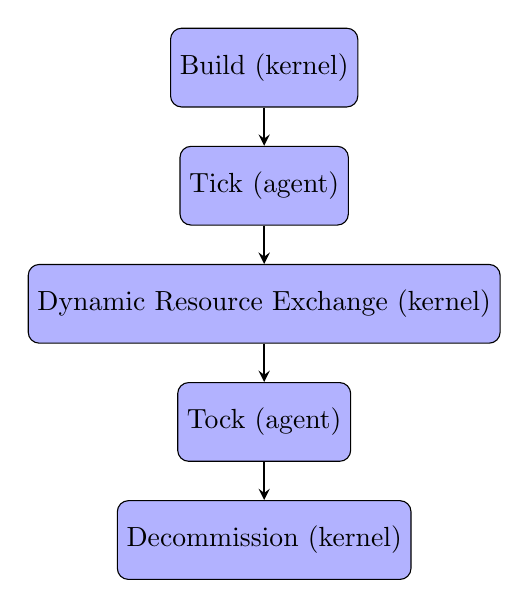
\begin{tikzpicture}[node distance=1.5cm]
\node (Build) [process] {Build (kernel)};
\node (Tick) [process, below of=Build] {Tick (agent)};
\node (DRE) [process, below of=Tick]{Dynamic Resource Exchange (kernel) };
\node (Tock) [process, below of=DRE]{Tock (agent)};
\node (Decom) [process, below of=Tock] {Decommission (kernel)};

\draw [arrow] (Build) -- (Tick); 
\draw [arrow] (Tick) -- (DRE);
\draw [arrow] (DRE) -- (Tock);
\draw [arrow] (Tock) -- (Decom);
\end{tikzpicture}
\caption{Each timestep in \Cyclus follows the five steps in order. Processes labeled
         kernel are executed by the \Cyclus framework, whereas processes labeled agent
         are executed by individual agents. What happens in the `Tick' and `Tock' is
         thus unique to each archetype.}
\label{diag:time}
\end{figure}


\section{Simulation parameter for Test Scenarios}
Simple parameters are given to fuel cycle facilities for the numerical testing of 
the algorithm.  \texttt{Source}, \texttt{Reactor} and \texttt{Sink} facilities are used in the test scenarios. 

Table \ref{tab:testscenario} provides basic parameters for each test scenario. 
Table \ref{tab:reactor} provides the parameters for the \texttt{Source},
\texttt{Reactor} and \texttt{Sink} in the test scenarios.

\begin{table}[H]
	\centering
	\caption {Basic Test Parameters}
	\label{tab:testscenario}
	\begin{tabular}{|l|l|l|}
		\hline
		\textbf{Test Scenario Parameters} & \textbf{Value} & \textbf{Units} \\
		\hline
		Duration & 15 & timesteps \\
		Timestep & 1 & month \\
		Start Month & 1 & month \\
		Start Year & 2000 & year \\
		\hline
	\end{tabular}
\end{table}

\begin{table}[H]
	\centering
    \caption {Source, Reactor and Sink Parameters}
	\label{tab:reactor}
	\begin{tabular}{|l|l|l|p{6.5cm}|}
\hline
\textbf{Source  Parameters} & \textbf{Value} & \textbf{Units} & \textbf{Description} \\
\hline
Throughput & 1 & kg & Quantity of output commodity the facility can output in one time step \\
\hline
Output Commodity & fuel & kg & The name of the output commodity\\
\hline
Lifetime & 7 & timesteps & Lifetime of the facility \\
\hline
Wait time & 2 & timesteps & Wait time for the facility to decommission when no longer needed \\
\hline
\textbf{Reactor Parameters} & \textbf{Value} & \textbf{Units} & \textbf{Description} \\
\hline
Input Commodity & fuel & kg & Name of input commodity\\
\hline
Output Commodity & spent\_uox & kg & Name of output commodity\\
\hline
Output Power Capacity & 1& MWe & MWe of power generated by reactor per operational timestep\\
\hline
Cycle Time & 1 & timestep & Duration of a full operational cycle of reactor\\
\hline
Refuel Time & 0 & timestep & Duration of a full refueling period \\
\hline
Lifetime & 7 & timestep & Lifetime of the facility \\
\hline
Wait time & 2 & timestep & Wait time for the facility to decommission when no longer needed \\
\hline
Assembly Size & 1 & & Quantity of commodity per assembly \\
\hline
Num. assemblies per batch & 1 & & Number of assemblies discharged and refueled per cycle\\
\hline
Num. assemblies per core & 3 & & Number of assemblies that make up the entire reactor core \\
\hline
Wait time & 2 & timestep & Wait time for the facility to decommission when no longer needed \\
\hline
\textbf{Sink Parameters} & \textbf{Value} & \textbf{Units}& \textbf{Description} \\
\hline
Input Commodity & spent\_uox & kg & Name of input commodity \\
\hline
Capacity & 5 & kg &Total amount of commodity it can hold \\
\hline
Lifetime & $\infty$ &timestep& Lifetime of the facility \\
\hline

Wait time & 2 &timestep& Wait time for the facility to decommission when no longer needed \\
\hline
	\end{tabular}
\end{table}

\pagebreak

\section{Numerical Tests for the Deterministic optimizing prediction method}
The deterministic optimizing prediction method is tested by comparing its output for various scenarios against their analytical solutions . In this section, the tests that must be met is described based on the parameters defined in table \ref{tab:testscenario} and \ref{tab:reactor} and analytical solution of a defined simple scenario. Unit test examples are included in Appendix B.

The tests are in forms of \texttt{[alphabet]-[traj]-[num]}. \texttt{Alphabet} refers to the supply chain of the test scenario,
\texttt{traj} the demand change in time, and \texttt{num} for tests with the same \texttt{alphabet} and \texttt{traj}.
\begin{itemize}
	\item \textbf{A} - Source $\rightarrow$ \texttt{End Demand Commodity}
	\item \textbf{B} - Source $\rightarrow$ Reactor $\rightarrow$ \texttt{End Demand Commodity}
	\item \textbf{C} - Source $\rightarrow$ Reactor $\rightarrow$ \texttt{End Demand Commodity} $\rightarrow$ Sink(disposal) 
\end{itemize}

Note that for test C, the \texttt{End Demand Commodity} is power generated from the reactor. The C tests additionally
check if the sink is deployed to meet spent fuel disposal demand.

The tests listed below are unique to the deterministic optimizing algorithm. The tests written in the non-optimizing algorithm report will also be used to test the deterministic optimizing algorithm but are not listed in this report.

The prediction algorithm for the deterministic optimizing method has three user-defined input parameters for the scenario.
The aim of the various test scenarios are to check if the
deterministic optimizing method archetype will deploy or decommission facilities correctly when there is a variation
in the combination of these input parameters. The input parameters are listed as an example in section \ref{sec:config}.

\begin{enumerate}
	\item End demand commodity
	\item Demand equation 
	\item Supply chain of facilities
\end{enumerate}

For each test scenario, there is one table that states the test scenario's input parameters and another table that states the exact analytical solution. In the latter table, there are columns specified for facilities "decommissioned" and "expired". Decommissioning refers to when the \texttt{Institution} removes the facility. Whereas expiring refers to when the facility's lifetime ends. 

Additionally, we created base tests that pass when the supply meets the demand within a given facility number tolerance.
In other words, when the supply exceeds the demand by the specified tolerance quantity, the test still passes. For this numerical experiment, the tolerance is set to one facility. 

\subsection{Test A-const-1}
The goal of test A-const-1 is to determine is a source facility is deployed when the lifetime of another is ending to meet the upcoming loss of power supply. 
Table \ref{tab:test_A-const-1} shows the input parameters of the \texttt{Institution} in the test scenario. Table \ref{tab:test_A-const-1ana} shows the expected analytical solution based on the test scenario. Table \ref{tab:test_A-const-1base} shows the accepted range of total number of facilities deployed and decommissioned over the test scenario which will pass the base test, which factors in the facility over or under prediction tolerance of 1.

\begin{figure}[H]
	\begin{center}
		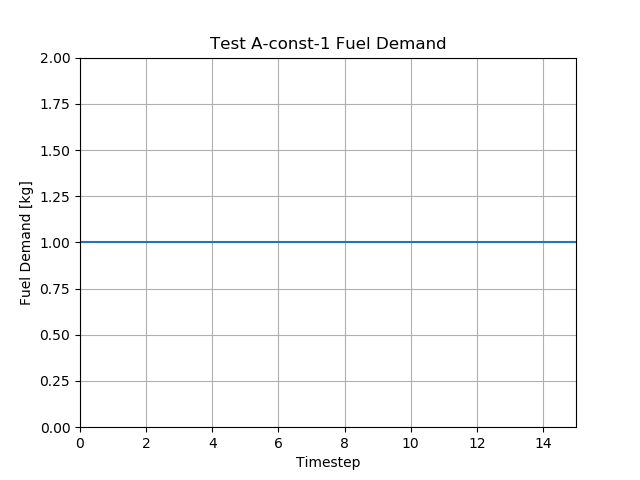
\includegraphics[scale=0.7]{./images/A-const-1.png}
	\end{center}
        \caption{Fuel demand for test A-const-1.}
	\label{fig:A-const-1}
\end{figure}


\begin{table}[H]
	\centering
	\caption{Test A-const-1 Scenario Input Parameters }
	\label{tab:test_A-const-1}
	\begin{tabular}{|l|l|l|}
		\hline
		\textbf{Input Parameter} & \textbf{Value} & \textbf{Units} \\
		\hline
		End demand commodity & fuel & kg \\
		Demand Equation & D = 1 & \\
		Supply Chain & source $\rightarrow$ \texttt{End Demand Commodity} &  \\
		\hline
	\end{tabular}
\end{table}


\begin{table}[H]
	\centering
	\caption{Test A-const-1 Analytical Solution (If the time step is skipped over, it is because there are no facilities deployed or decommissioned during that time step.)}
	\label{tab:test_A-const-1ana}
	\begin{tabular}{|l|l|l|l|}
		\hline
		\textbf{Time Step} & \textbf{\shortstack{No. of Source \\ Deployed}} & \textbf{\shortstack{No. of Source \\ Decommissioned}} & \textbf{\shortstack{No. of Source \\ Expired}} \\
		\hline
		1 & 0 & 1 & 0 \\
		7 & 0 & 0 & 1 \\
		8 & 0 & 1 & 0 \\
		14 & 0 & 0 & 1 \\
		15 & 0 & 1 & 0 \\
		\hline
	\end{tabular}
\end{table}

\begin{table}[H]
	\centering
	\caption{Test A-const-1 Base Test Acceptance}
	\label{tab:test-A-const-1base}
	\begin{tabular}{|P{7.5cm}|}
		\hline
		\textbf{\shortstack{Acceptable total No. of Source \\Facilities Deployed + tolerance}}\\
		\hline
		3 $<$ x $<$ 4 \\
		\hline
	\end{tabular}
\end{table}

\subsection{Test A-const-2}
The goal of test A-const-2 is to determine whether a source facility is deployed
to meet the upcoming loss of supply due to the end of a lifetime of another.
The difference between this test and test A-const-1 is that multiple facilities
exit and are deployed at different times.
Table \ref{tab:test-A-const-2} shows the input parameters of the \texttt{Institution}. Table \ref{tab:test-A-const-2ana} shows the expected analytical solution based on the test scenario. Table \ref{tab:test-A-const-2base} shows the accepted range of total number of facilities deployed and decommissioned over the test scenario which will pass the base test, which factors in the facility over or under prediction tolerance of 1.

\begin{figure}[H]
	\begin{center}
		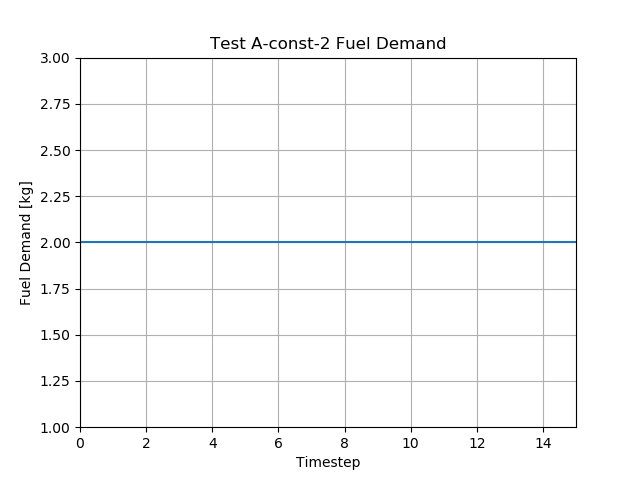
\includegraphics[scale=0.7]{./images/A-const-2.png}
	\end{center}
        \caption{Fuel demand for test A-const-2.}
	\label{fig:A-dep-2}
\end{figure}

\begin{table}[H]
	\centering
	\caption{Test A-const-2 Scenario Input Parameters }
	\label{tab:test_A-const-2}
	\begin{tabular}{|l|l|l|}
		\hline
		\textbf{Input Parameter} & \textbf{Value} & \textbf{Units} \\
		\hline
		End demand commodity & fuel & kg \\
		Demand Equation & D = 2 & \\
		Supply Chain & source $\rightarrow$ \texttt{End Demand Commodity} &  \\
		\hline
	\end{tabular}
\end{table}s

\begin{table}[H]
	\centering
	\caption{Test A-const-2 Analytical Solution (If the time step is skipped over, it is because there
			 are no facilities deployed or decommissioned during that time step.)}
	\label{tab:test-A-const-2ana}
	\begin{tabular}{|l|l|l|l|}
		\hline
		\textbf{Time Step} & \textbf{\shortstack{No. of Source \\ Deployed}} & \textbf{\shortstack{No. of Source \\ Decommissioned}} & \textbf{\shortstack{No. of Source \\ Expired}} \\
		\hline
		0 & 1 & 0 & 0 \\
		1 & 1 & 0 & 0 \\
		6 & 0 & 0 & 1 \\
		7 & 1 & 0 & 1 \\
		8 & 1 & 0 & 0 \\
		13 & 0 & 0 & 1 \\
		14 & 1 & 0 & 1 \\
		15 & 1 & 0 & 0 \\
		\hline
	\end{tabular}
\end{table}

\begin{table}[H]
	\centering
	\caption{Test A-const-2 Base Test Acceptance}
	\label{tab:test-A-const-2 base}
	\begin{tabular}{|P{7.5cm}|}
		\hline
		\textbf{\shortstack{Acceptable total No. of Source \\Facilities Deployed + tolerance}}\\
		\hline
		6 $<$ x $<$ 7 \\
		\hline
	\end{tabular}
\end{table}

\subsection{Test A-grow-1}
The goal of test A-grow-1 is to determine whether source facilities are deployed
to meet the increasing fuel demand. 
Table \ref{tab:test-A-grow-1} shows the input parameters of the \texttt{Institution}. Table \ref{tab:test-A-grow-1ana} shows the expected analytical solution based on the test scenario. Table \ref{tab:test-A-grow-1base} shows the accepted range of total number of facilities deployed and decommissioned over the test scenario which will pass the base test, which factors in the facility over or under prediction tolerance of 1.

\begin{figure}[H]
	\begin{center}
		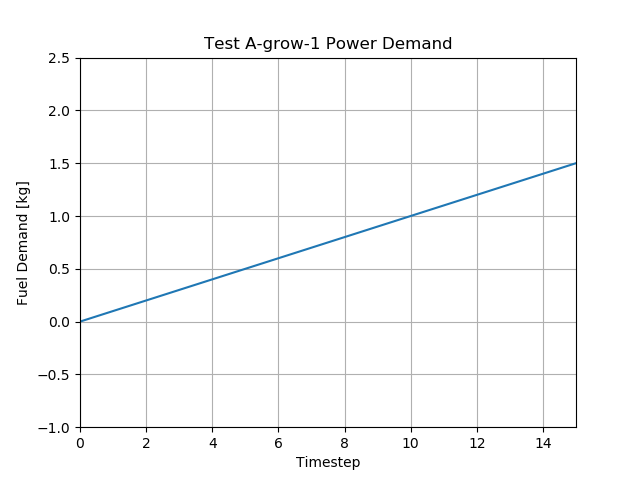
\includegraphics[scale=0.7]{./images/A-grow-1.png}
	\end{center}
	\caption{Fuel demand for test A-grow-1.}
	\label{fig:A-grow-1}
\end{figure}

\begin{table}[H]
	\centering
	\caption{Test A-grow-1 Scenario Input Parameters }
	\label{tab:test_A-grow-1}
	\begin{tabular}{|l|l|l|}
		\hline
		\textbf{Input Parameter} & \textbf{Value} & \textbf{Units} \\
		\hline
		End demand commodity & fuel & kg \\
		Demand Equation & $D = 0.1 \times timestep $& \\
		Supply Chain & source $\rightarrow$ \texttt{End Demand Commodity} &  \\
		\hline
	\end{tabular}
\end{table}

\begin{table}[H]
	\centering
	\caption{Test A-grow-1 Analytical Solution (If the time step is skipped over, it is because there
		are no facilities deployed or decommissioned during that time step.)}
	\label{tab:test-A-grow-1ana}
	\begin{tabular}{|l|l|l|l|}
		\hline
		\textbf{Time Step} & \textbf{\shortstack{No. of Source \\ Deployed}} & \textbf{\shortstack{No. of Source \\ Decommissioned}} & \textbf{\shortstack{No. of Source \\ Expired}} \\
		\hline
		1 & 1 & 0 & 0 \\
		7 & 0 & 0 & 1 \\
		8 & 1 & 0 & 0 \\
		11 & 1 & 0 & 0 \\
		14 & 0 & 0 & 1 \\
		15 & 1 & 0 & 0 \\
		\hline
	\end{tabular}
\end{table}

\begin{table}[H]
	\centering
	\caption{Test A-grow-1 Base Test Acceptance}
	\label{tab:test-A-grow-1 base}
	\begin{tabular}{|P{7.5cm}|}
		\hline
		\textbf{\shortstack{Acceptable total No. of Source \\Facilities Deployed + tolerance}}\\
		\hline
		4 $<$ x $<$ 5 \\
		\hline
	\end{tabular}
\end{table}

\subsection{Test A-decl-1}
The goal of test A-decl-1 is to determine if a source facility is not decommissioned until after the wait time (defined in Table \ref{tab:reactor}) even if there is over-supply of fuel commodity. Figure \ref{fig:A-decl-1} shows the plot of the fuel demand for test A-decl-1. 
Table \ref{tab:testA-decl-1} shows the input parameters of the \texttt{Institution} in the test scenario. Table \ref{tab:testA-decl-1ana} shows the expected analytical solution based on the test scenario. 

\begin{table}[H]
	\centering
	\caption{Test A-decl-1 Scenario Input Parameters }
	\label{tab:test_A-decl-1}
	\begin{tabular}{|l|l|l|}
		\hline
		\textbf{Input Parameter} & \textbf{Value} & \textbf{Units} \\
		\hline
		End demand commodity & fuel & kg \\
		Demand Equation & $D = \left\{
		\begin{array}{ll}
			1 , & 0 < t < 2 \\
			0 , &  2 \leq t  \\
		\end{array}\right\}$
		& \\
		Supply Chain & source $\rightarrow$ \texttt{End Demand Commodity} &  \\
		\hline
		\end{tabular}
\end{table}

\begin{figure}[H]
	\begin{center}
				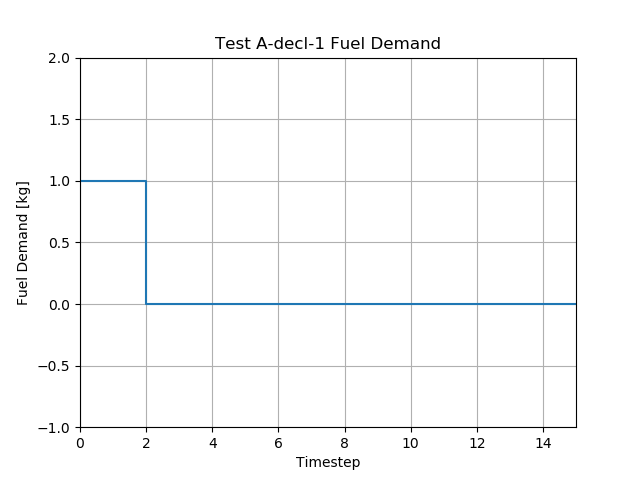
\includegraphics[scale=0.7]{./images/A-decl-1.png}
	\end{center}
	\caption{Fuel demand for test A-decl-1.}
	\label{fig:A-decl-1}
\end{figure}

\begin{table}[H]
	\centering
	\caption{Test A-decl-1 Analytical Solution (If the time step is skipped over, it is because there are no facilities deployed or decommissioned during that time step.)}
	\label{tab:testA-decl-1ana}
	\begin{tabular}{|l|l|l|l|}
		\hline
		\textbf{Time Step} & \textbf{\shortstack{No. of Source \\ Deployed}} & \textbf{\shortstack{No. of Source \\ Decommissioned}} & \textbf{\shortstack{No. of Source \\ Expired}} \\
		\hline
		1 & 1 & 0 & 0\\
		5 & 0 & 1 & 0\\
		\hline
	\end{tabular}
\end{table}

\subsection{Test A-decl-2}
The goal of test A-decl-2 is to determine if a source facilities decommissions as fuel demand decreases while obeying the wait time (defined in Table \ref{tab:reactor}) even if there is over-supply of fuel commodity. Figure \ref{fig:A-decl-2} shows the plot of the fuel demand for test A-decl-2. 
Table \ref{tab:testA-decl-2} shows the input parameters of the \texttt{Institution} in the test scenario. Table \ref{tab:testA-decl-2ana} shows the expected analytical solution based on the test scenario. 

\begin{table}[H]
	\centering
	\caption{Test A-decl-2 Scenario Input Parameters }
	\label{tab:testA-decl-2}
	\begin{tabular}{|l|l|l|}
		\hline
		\textbf{Input Parameter} & \textbf{Value} & \textbf{Units} \\
		\hline
		End demand commodity & fuel & kg \\
		Demand Equation & $D = -0.1 \times timestep + 2$ & \\
		Supply Chain & source $\rightarrow$ \texttt{End Demand Commodity} &  \\
		\hline
	\end{tabular}
\end{table}

\begin{figure}[H]
	\begin{center}
		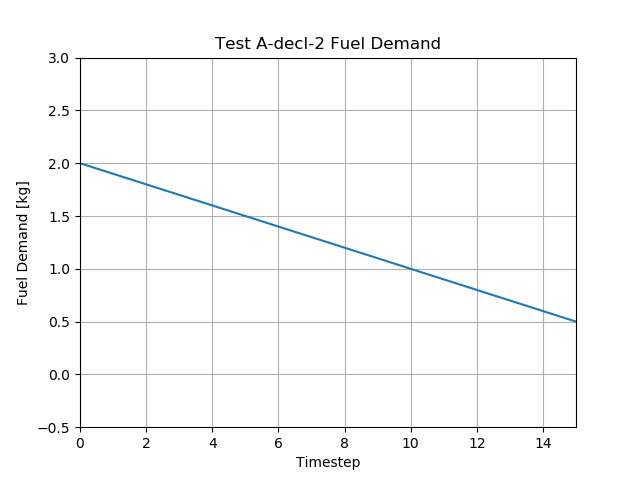
\includegraphics[scale=0.7]{./images/A-decl-2.png}
	\end{center}
	\caption{Fuel demand for test A-decl-2.}
	\label{fig:A-decl-2}
\end{figure}

\begin{table}[H]
	\centering
	\caption{Test A-decl-2 Analytical Solution (If the time step is skipped over, it is because there are no facilities deployed or decommissioned during that time step.)}
	\label{tab:testA-decl-2ana}
	\begin{tabular}{|l|l|l|l|}
		\hline
		\textbf{\shortstack{Time \\ Step}} & \textbf{\shortstack{No. of Sources \\ Deployed}} & \textbf{\shortstack{No. of Sources \\ Decommissioned}} & \textbf{\shortstack{No. of \\ Sources Expire}} \\
		\hline
		1 & 2 & 0 & 0 \\
		7 & 0 & 0 & 2 \\
		8 & 2 & 0 & 0 \\
		13 & 0 & 1 & 0 \\
		14 & 0 & 0 & 1 \\
		15 & 1 & 0 & 0 \\
		\hline
	\end{tabular}
\end{table}

\subsection{Test A-mix-1}
The goal of test A-mix-1 is to determine if a source facilities deploy and decommission as fuel demand changes while obeying the wait time (defined in Table \ref{tab:reactor}) even if there is over-supply of fuel commodity. Figure \ref{fig:A-mix-1} shows the plot of the fuel demand for test A-mix-1. 
Table \ref{tab:testA-mix-1} shows the input parameters of the \texttt{Institution} in the test scenario. Table \ref{tab:testA-mix-1ana} shows the expected analytical solution based on the test scenario. 

\begin{table}[H]
	\centering
	\caption{Test A-mix-1 Scenario Input Parameters }
	\label{tab:testA-mix-1}
	\begin{tabular}{|l|l|l|}
		\hline
		\textbf{Input Parameter} & \textbf{Value} & \textbf{Units} \\
		\hline
		End demand commodity & fuel & kg \\
		Demand Equation & $D = \left\{
		\begin{array}{ll}
		0.5 \times t , & 0 \leq t \leq  6 \\
		-0.2 \times t +4.2 , &  6 \leq t \leq  15  \\
		\end{array}\right\}$
		& \\
		Supply Chain & source $\rightarrow$ \texttt{End Demand Commodity} &  \\
		\hline
	\end{tabular}
\end{table}

\begin{figure}[H]
	\begin{center}
		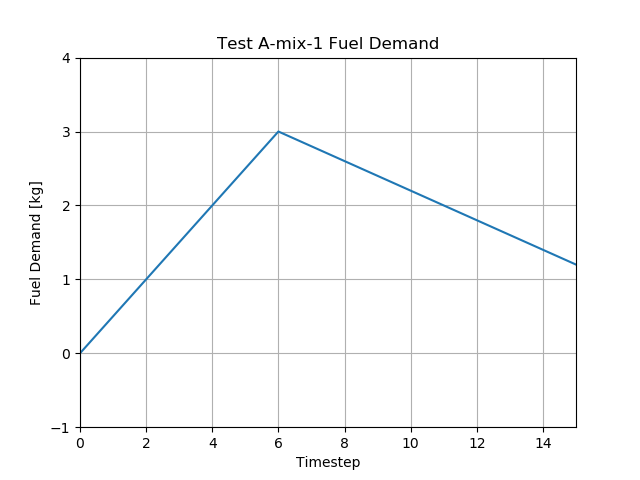
\includegraphics[scale=0.7]{./images/A-mix-1.png}
	\end{center}
	\caption{Fuel demand for test A-mix-1.}
	\label{fig:A-mix-1}
\end{figure}

\begin{table}[H]
	\centering
	\caption{Test A-mix-1 Analytical Solution (If the time step is skipped over, it is because there are no facilities deployed or decommissioned during that time step.)}
	\label{tab:testA-mix-1ana} 
	\begin{tabular}{|l|l|l|l|}
		\hline
		\textbf{Time Step} & \textbf{\shortstack{No. of Source \\ Deployed}} & \textbf{\shortstack{No. of Source \\ Decommissioned}} & \textbf{\shortstack{No. of Source \\ Expired}} \\
		\hline
		1 & 1 & 0 & 0  \\
		3 & 1 & 0 & 0  \\
		5 & 1 & 0 & 0  \\
		7 & 0 & 0 & 1  \\
		8 & 1 & 0 & 0  \\
		9 & 0 & 0 & 1  \\
		10 & 1 & 0 & 0  \\
		11 & 0 & 0 & 1  \\
		14 & 0 & 0 & 1  \\
		15 & 1 & 0 & 0  \\
		\hline
	\end{tabular}
\end{table}

\subsection{Test B-const-1}
The goal of test B-const-1 is to determine if source and reactor facilities are deployed when the lifetime of another is ending. Figure \ref{fig:B-const-1} shows the plot of the power demand for test B-const-1. 
Table \ref{tab:testB-const-1} shows the input parameters of the \texttt{Institution} in the test scenario. Figure \ref{fig:B-const-1} shows the plot of the fuel demand for test B-const-1. 
Table \ref{tab:testB-const-1ana} shows the expected analytical solution based on the test scenario. Table \ref{tab:testB-const-1base} shows the accepted range of total number of facilities deployed over the test scenario which will pass the base test, which factors in the facility over prediction tolerance of 1. 

\begin{table}[H]
	\centering
	\caption{Test B-const-1 Scenario Input Parameters }
	\label{tab:test_B-const-1}
	\begin{tabular}{|l|l|l|}
		\hline
		\textbf{Input Parameter} & \textbf{Value} & \textbf{Units} \\
		\hline
		End demand commodity & Power & MWe \\
		Demand Equation & D = 1 & \\
		Supply Chain & source $\rightarrow$ reactor $\rightarrow$ \texttt{End Demand Commodity} &  \\
		\hline
	\end{tabular}
\end{table}

\begin{figure}[H]
	\begin{center}
		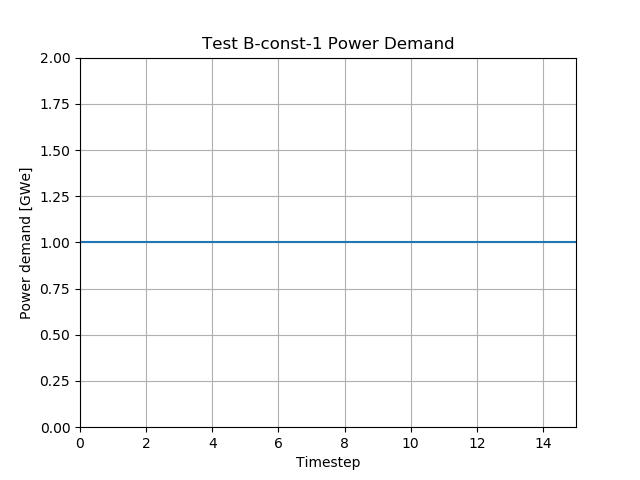
\includegraphics[scale=0.7]{./images/B-const-1.png}
	\end{center}
	\caption{Power demand for test B-const-1.}
	\label{fig:B-const-1}
\end{figure}

\begin{table}[H]
	\centering
	\caption{Test B-const-1 Analytical Solution}
	\label{tab:testB-const-1ana}
	\begin{tabular}{|l|l|l|l|l|l|l|}
		\hline
		\textbf{\shortstack{Time \\ Step}} & \textbf{\shortstack{No. of \\ Source \\ Deployed}} & \textbf{\shortstack{No. of \\ Reactor \\ Deployed}} & \textbf{\shortstack{No. of \\ Source \\ Decom}}& \textbf{\shortstack{No. of \\ Reactor \\ Decom}}& \textbf{\shortstack{No. of \\ Sources \\Expired}} & \textbf{\shortstack{No. of \\ Reactors \\Expired}} \\
		\hline
		1 & 3 & 1 &0&0& 0 & 0 \\
		7 & 0 & 0 &0&0 & 3 & 1 \\
		8 & 3 & 1 &0&0& 0 & 0 \\
		14 & 0 & 0 &0&0 & 3 & 1 \\
		15  & 3 & 1 &0&0& 0 & 0 \\
		\hline
	\end{tabular}
\end{table}

\begin{table}[H]
	\centering
	\caption{Test B-const-1 Base Test Acceptance}
	\label{tab:testB-const-1base}
	\begin{tabular}{|P{6.5cm}|P{6.5cm}|}
		\hline
		\textbf{\shortstack{Acceptable total No. of Source \\Facilities Deployed + tolerance}} &\textbf{\shortstack{Acceptable total No. of Reactor \\Facilities Deployed + tolerance}}\\
		\hline
		9 $<$ x $<$ 10 & 3 $<$ x $<$ 4\\
		\hline
	\end{tabular}
\end{table}


\subsection{Test B-grow-1}
The goal of test B-grow-1 is to determine whether source and reactor facilities are deployed
to meet the increasing power demand. 
Table \ref{tab:test-B-grow-1} shows the input parameters of the \texttt{Institution}. Table \ref{tab:test-B-grow-1ana} shows the expected analytical solution based on the test scenario. Table \ref{tab:test-B-grow-1base} shows the accepted range of total number of facilities deployed and decommissioned over the test scenario which will pass the base test, which factors in the facility over or under prediction tolerance of 1.

\begin{table}[H]
	\centering
	\caption{Test B-grow-1 Scenario Input Parameters }
	\label{tab:test_B-grow-1}
	\begin{tabular}{|l|l|l|}
		\hline
		\textbf{Input Parameter} & \textbf{Value} & \textbf{Units} \\
		\hline
		End demand commodity & Power & GWe \\
		Demand Equation & D = 0.1 * t & \\
		Supply Chain & source $\rightarrow$ reactor $\rightarrow$ \texttt{End Demand Commodity} &  \\
		\hline
	\end{tabular}
\end{table}

\begin{figure}[H]
	\begin{center}
		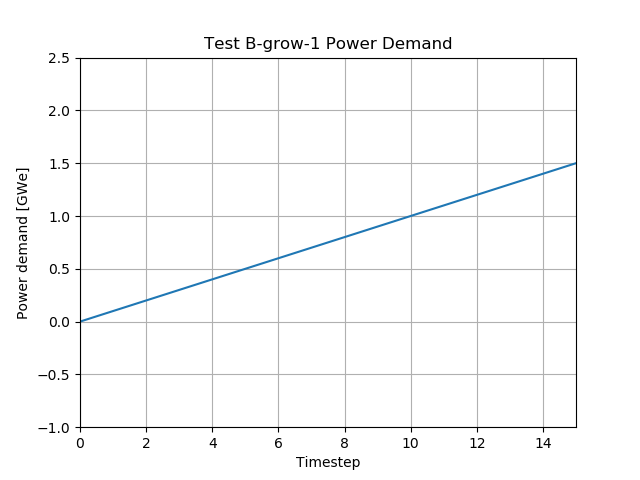
\includegraphics[scale=0.7]{./images/B-grow-1.png}
	\end{center}
	\caption{Power demand for test B-grow-1.}
	\label{fig:B-grow-1}
\end{figure}

\begin{table}[H]
	\centering
	\caption{Test B-grow-1 Analytical Solution}
	\label{tab:testB-grow-1ana}
	\begin{tabular}{|l|l|l|l|l|}
		\hline
		\textbf{Time Step} & \textbf{\shortstack{No. of \\ Source \\ Deployed}} & \textbf{\shortstack{No. of \\ Reactor \\ Deployed}} & \textbf{\shortstack{No. of \\ Sources \\Expire}} & \textbf{\shortstack{No. of \\ Reactors \\Expire}} \\
		\hline
		1 & 3 & 1 & 0 & 0 \\
		7 & 0 & 0  & 3 & 1 \\
		8 & 3 & 1 & 0 & 0 \\
		11 & 3 & 1 & 0 & 0 \\
		14 & 0 & 0  & 3 & 1 \\
		15  & 3 & 1 & 0 & 0 \\
		\hline
	\end{tabular}
\end{table}

\begin{table}[H]
	\centering
	\caption{Test B-grow-1 Base Test Acceptance}
	\label{tab:test-B-grow-1base}
	\begin{tabular}{|P{6.5cm}|P{6.5cm}|}
		\hline
		\textbf{\shortstack{Acceptable total No. of Source \\Facilities Deployed + tolerance}} &\textbf{\shortstack{Acceptable total No. of Reactor \\Facilities Deployed + tolerance}}\\
		\hline
		12 $<$ x $<$ 13 & 4 $<$ x $<$ 5\\
		\hline
	\end{tabular}
\end{table}


%%%%%%%%%%%%%%%%%%%%%%%%%%%%%%%%%%%%%%%%%%%%%%%%%%%%%%%%%%%%%
\subsection{Test B-decl-1}
The goal of test B-decl-1 is to determine whether source and reactor facilities are controlled
to meet decreasing demand.
Table \ref{tab:test-B-decl-1} shows the input parameters of the \texttt{Institution}. Table \ref{tab:test-B-decl-1ana} shows the expected analytical solution based on the test scenario. Table \ref{tab:test-B-decl-1base} shows the accepted range of total number of facilities deployed and decommissioned over the test scenario which will pass the base test, which factors in the facility over or under prediction tolerance of 1.

\begin{table}[H]
	\centering
	\caption{Test B-decl-1 Scenario Input Parameters }
	\label{tab:test_B-decl-1}
	\begin{tabular}{|l|l|l|}
		\hline
		\textbf{Input Parameter} & \textbf{Value} & \textbf{Units} \\
		\hline
		End demand commodity & Power & GWe \\
		Demand Equation & D = 2 - (0.1 * t) & \\
		Supply Chain & source $\rightarrow$ reactor $\rightarrow$ \texttt{End Demand Commodity} &  \\
		\hline
	\end{tabular}
\end{table}

\begin{figure}[H]
	\begin{center}
		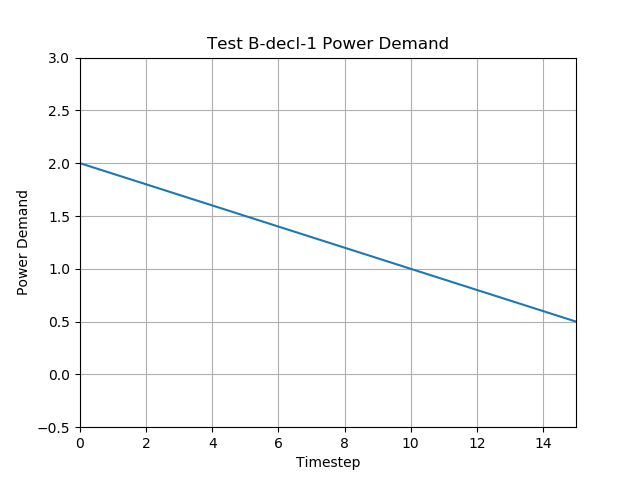
\includegraphics[scale=0.7]{./images/B-decl-1.png}
	\end{center}
	\caption{Power demand for test B-decl-1.}
	\label{fig:B-decl-1}
\end{figure}

\begin{table}[H]
	\centering
	\caption{Test B-decl-1 Analytical Solution}
	\label{tab:testB-decl-1ana}
	\begin{tabular}{|l|l|l|l|l|l|l|}
		\hline
		\textbf{\shortstack{Time \\ Step}} & \textbf{\shortstack{No. of \\ Source \\ Deployed}} & \textbf{\shortstack{No. of \\ Reactor \\ Deployed}} & \textbf{\shortstack{No. of \\ Source \\ Decom}}& \textbf{\shortstack{No. of \\ Reactor \\ Decom}}& \textbf{\shortstack{No. of \\ Sources \\Expired}} & \textbf{\shortstack{No. of \\ Reactors \\Expired}} \\
		\hline
		1 & 6 & 2 &0&0& 0 & 0 \\
		7 & 0 & 0  &0&0& 6 & 2 \\
		8 & 6 & 2 &0&0& 0 & 0 \\
		13 & 0 & 0 &3&1& 0 & 0 \\
		14 & 0 & 0  &0&0& 3 & 1 \\
		15  & 3 & 1 &0&0& 0 & 0 \\
		\hline
	\end{tabular}
\end{table}

\begin{table}[H]
	\centering
	\caption{Test B-decl-1 Base Test Acceptance}
	\label{tab:test-B-decl-1base}
	\begin{tabular}{|P{6.5cm}|P{6.5cm}|}
		\hline
		\textbf{\shortstack{Acceptable total No. of Source \\Facilities Deployed + tolerance}} &\textbf{\shortstack{Acceptable total No. of Reactor \\Facilities Deployed + tolerance}}\\
		\hline
		15 $<$ x $<$ 16 & 5 $<$ x $<$ 6\\
		\hline
	\end{tabular}
\end{table}


%%%%%%%%%%%%%%%%%%%%%%%%%%%%%%%%%%%%%%%
\subsection{Test B-mix-1}
The goal of test B-mix-1 is to determine whether source and reactor facilities are controlled
to meet increasing and decreasing demand.
Table \ref{tab:test-B-mix-1} shows the input parameters of the \texttt{Institution}. Table \ref{tab:test-B-mix-1ana} shows the expected analytical solution based on the test scenario. Table \ref{tab:test-B-mix-1base} shows the accepted range of total number of facilities deployed and decommissioned over the test scenario which will pass the base test, which factors in the facility over or under prediction tolerance of 1.

\begin{table}[H]
	\centering
	\caption{Test B-mix-1 Scenario Input Parameters }
	\label{tab:test_B-mix-1}
	\begin{tabular}{|l|l|l|}
		\hline
		\textbf{Input Parameter} & \textbf{Value} & \textbf{Units} \\
		\hline
		End demand commodity & Power & GWe \\
		Demand Equation & $D = \left\{
		\begin{array}{ll}
		0.5 * t , & 0 < t \leq 6 \\
		4.2 - 0.2 *t, &  6 < t  \\
		\end{array}\right\}$ & \\
		Supply Chain & source $\rightarrow$ reactor $\rightarrow$ \texttt{End Demand Commodity} &  \\
		\hline
	\end{tabular}
\end{table}

\begin{figure}[H]
	\begin{center}
		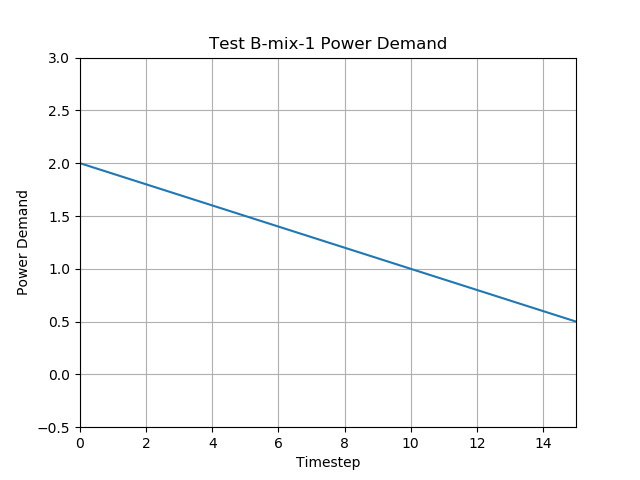
\includegraphics[scale=0.7]{./images/B-mix-1.png}
	\end{center}
	\caption{Power demand for test B-mix-1.}
	\label{fig:B-mix-1}
\end{figure}

\begin{table}[H]
	\centering
	\caption{Test B-mix-1 Analytical Solution}
	\label{tab:testB-mix-1ana}
	\begin{tabular}{|l|l|l|l|l|l|l|}
		\hline
		\textbf{\shortstack{Time \\ Step}} & \textbf{\shortstack{No. of \\ Source \\ Deployed}} & \textbf{\shortstack{No. of \\ Reactor \\ Deployed}} & \textbf{\shortstack{No. of \\ Source \\ Decom}}& \textbf{\shortstack{No. of \\ Reactor \\ Decom}}& \textbf{\shortstack{No. of \\ Sources \\Expired}} & \textbf{\shortstack{No. of \\ Reactors \\Expired}} \\
		\hline
		1 & 3 & 1 &0&0& 0 & 0 \\
		3 & 3 & 1 &0&0& 0 & 0 \\
		5 & 3 & 1 &0&0& 0 & 0 \\
		7 & 0 & 0 &0&0& 3 & 1 \\
		8 & 3 & 1 &0&0& 0 & 0 \\
		9 & 0 & 0 &0&0& 3 & 1 \\
		10 & 3 & 1 &0&0& 0 & 0 \\
		11 & 0 & 0 &0&0& 3 & 1 \\
		14 & 0 & 0 &0&0& 3 & 1 \\
		15 & 3 & 1 &0&0& 0 & 0 \\
		\hline
	\end{tabular}
\end{table}

\begin{table}[H]
	\centering
	\caption{Test B-mix-1 Base Test Acceptance}
	\label{tab:test-B-mix-1base}
	\begin{tabular}{|P{6.5cm}|P{6.5cm}|}
		\hline
		\textbf{\shortstack{Acceptable total No. of Source \\Facilities Deployed + tolerance}} &\textbf{\shortstack{Acceptable total No. of Reactor \\Facilities Deployed + tolerance}}\\
		\hline
		18 $<$ x $<$ 19 & 6 $<$ x $<$ 7\\
		\hline
	\end{tabular}
\end{table}



%%%%%%%%%%%%%%%%%%%
\subsection{Test C-const-1}
Test C-const-1 tests three capabilities:
\begin{enumerate}
	\item Deployment of reactors to meet power demand
	\item Deployment of sources to meet fuel demand for reactor
	\item Deployment of sinks to meet spent fuel disposal demand
\end{enumerate}

Table \ref{tab:test-C-const-1} shows the input parameters of the \texttt{Institution}. Table \ref{tab:test-C-const-1ana} shows the expected analytical solution based on the test scenario. Table \ref{tab:test-C-const-1base} shows the accepted range of total number of facilities deployed and decommissioned over the test scenario which will pass the base test, which factors in the facility over or under prediction tolerance of 1.

\begin{table}[H]
	\centering
	\caption{Test C-const-1 Scenario Input Parameters }
	\label{tab:test_C-const-1}
	\begin{tabular}{|l|l|l|}
		\hline
		\textbf{Input Parameter} & \textbf{Value} & \textbf{Units} \\
		\hline
		End demand commodity & Power & GWe \\
		Demand Equation & D = 1 & \\
		Supply Chain & source $\rightarrow$ reactor $\rightarrow$ \texttt{End Demand Commodity} &  \\
		Supply Chain 2 & source $\rightarrow$ reactor $\rightarrow$ sink (disposal) & \\
		\hline
	\end{tabular}
\end{table}

\begin{figure}[H]
	\begin{center}
		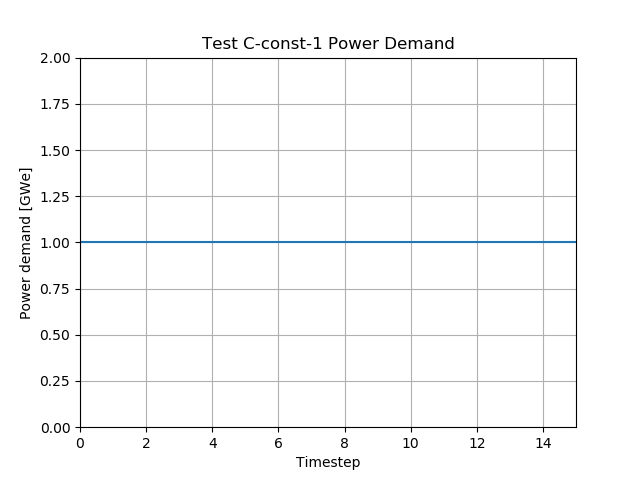
\includegraphics[scale=0.7]{./images/C-const-1.png}
	\end{center}
	\caption{Power demand for test C-const-1.}
	\label{fig:C-const-1}
\end{figure}

\begin{figure}[H]
	\begin{center}
		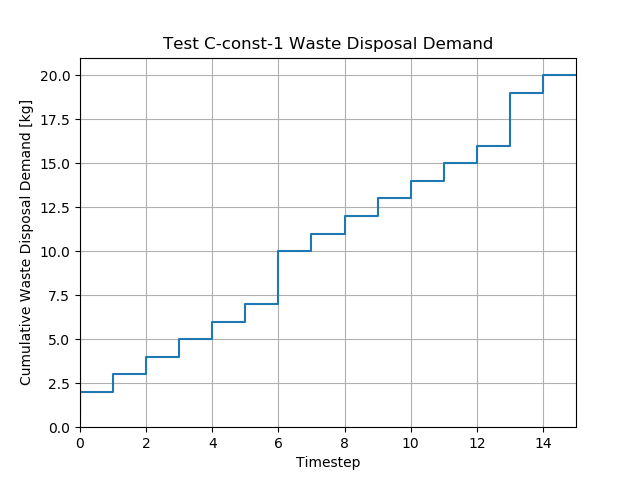
\includegraphics[scale=0.7]{./images/C-const-1-waste.png}
	\end{center}
	\caption{Waste Disposal demand for test C-const-1.}
	\label{fig:C-const-1-waste}
\end{figure}


\begin{table}[H]
	\centering
	\caption{Test C-const-1 Analytical Solution}
	\label{tab:testC-const-1ana}
	\begin{tabular}{|l|l|l|l|l|l|l|l|}
		\hline
		\textbf{\shortstack{Time \\ Step}} & \textbf{\shortstack{No. of \\ Source \\ Deployed}} & \textbf{\shortstack{No. of \\ Reactor \\ Deployed}} & \textbf{\shortstack{No. of \\ Sink \\ Deployed}} &  \textbf{\shortstack{No. of \\ Source \\ Decom}}& \textbf{\shortstack{No. of \\ Reactor \\ Decom}}& \textbf{\shortstack{No. of \\ Sources \\Expired}} & \textbf{\shortstack{No. of \\ Reactors \\Expired}} \\
		1 & 3 & 1 & 1 & 0 & 0 & 0 & 0 \\
		6 & 0 & 0 & 1 & 0 & 0 & 0 & 0\\
		7 & 0 & 0 & 0 & 0 & 0 & 3 & 1\\
		8 & 3 & 1 & 0 & 0 & 0 & 0 & 0\\
		9 & 0 & 0 & 1 & 0 & 0 & 0 & 0\\
		14 & 0 & 0 & 1 & 0 & 0 & 3 & 1\\
		\hline
		\hline
	\end{tabular}
\end{table}


\begin{table}[H]
	\centering
	\caption{Test C-const-1 Base Test Acceptance}
	\label{tab:test-C-const-1base}
	\begin{tabular}{|P{4.7cm}|P{4.7cm}|P{4.7cm}|}
		\hline
		\textbf{\shortstack{Acceptable total No. of \\ Source Deployed + tol}} &\textbf{\shortstack{Acceptable total No. of \\ Reactor Deployed + tol}} & \textbf{\shortstack{Acceptable total No. of \\ Deployed + tol}}\\
		\hline
		6 $<$ x $<$ 7 & 2 $<$ x $<$ 3 & 4 $<$ x $<$ 5\\
		\hline
	\end{tabular}
\end{table}

\section{Numerical Test Results}


\section{References}
\bibliography{bibliography}

\section*{Appendix A - parameter configuration}

\section*{Appendix B - Sample Test Code }

\section*{Appendix C - Numerical Experiment Solution for test scenarios}

\end{document}



